\section*{Úkol 1}
\label{sec:task-1}

Pomocí nástrojů explorační analýzy zkoumejte nárůst výkonnostních skóre (FPS) po aplikaci 1.5 patche 
(tj. rozdíl výkonnostních skóre pro verzi „patched“ a verzi „release“) ve hře "Cyberpunk 2077" pro grafické karty 
\nvidiaCard\ a \amdCard\. Data vhodně graficky prezentujte (krabicový graf, histogram, q-q graf)
a doplňte následující tabulku a text.

\vspace{2em}
\noindent
Výsledky popisné statistiky lze vidět v \tabref{tab:characteristics-summary} a na  \figref{fig:box_plot}, \figref{fig:histogram} a \figref{fig:qq}.

% Fill your table values here :)
\newcommand{\rangeValues}       {70,        59,         69,         58}
\newcommand{\minValues}         {-4.8,      4.2,        5.1,        4.2}
\newcommand{\QfValues}          {5.425,     4.900,      5.500,      4.900}
\newcommand{\medianValues}      {5.700,     5.300,      5.700,      5.300}
\newcommand{\meanValues}        {5.600,     5.371,      5.750,      5.191}
\newcommand{\QtValues}          {6.100,     5.550,      6.100,      5.500}
\newcommand{\maxValues}         {6.6,       15.8,       6.6,        5.9}
\newcommand{\sdValues}          {1.335,     1.452,      0.439,      0.451}
\newcommand{\cvValues}          {23.8,      27.0,       7.6,        8.7}
\newcommand{\skewnessValues}    {-6.9,      6.4,        0.2,        -0.4}
\newcommand{\kurtosisValues}    {51.3,      43.8,       -1.0,       -0.7}
\newcommand{\lowerBoundValues}  {4.41,      3.92,       0,          0}
\newcommand{\upperBoundValues}  {7.11,      6.52,       0,          0}

% Additional values
\newcommand{\sigmaValues} {4.873, 6.628, 4.289, 6.093}

% Helper command to put everything in table.
\newcommand{\tableValue}[2]{%
    \pgfmathparse{{#1}[#2]}%
    \edef\tempResult{\pgfmathresult}%
    \ifnum\pdfstrcmp{\tempResult}{inf}=0 %
        $\infty$%
    \else%
        \mbox{\tempResult}%
    \fi%
}

% Fuckin graphic card names
\newcommand{\nvidiaCard}{Nvidia RTX 3070 Ti}
\newcommand{\amdCard} {AMD Radeon RX 7700 XT}

\begin{table}[h!]
    \caption{Nárůst výkonnostních skóre (FPS) po aplikaci 1.5 patche ve hře "Cyberpunk 2077" pro grafické karty \nvidiaCard\ a \amdCard\ (souhrnné statistiky)}
    \label{tab:characteristics-summary}
    \vspace{0.5em}
    \renewcommand{\arraystretch}{1.3}
    \resizebox{\textwidth}{!}{%
        \begin{tabular}{|p{3.5cm}|P{3cm}|P{3cm}|P{3cm}|P{3cm}|}
            \hline
                                  & \multicolumn{2}{P{6cm}|}{\textbf{Původní data}}                   & \multicolumn{2}{P{6cm}|}{\textbf{Data po odstranění odlehlých pozorování}} \\ \hline
                                  & \centering \textbf{\nvidiaCard} & \textbf{\amdCard}               & \centering \textbf{\nvidiaCard} & \textbf{\amdCard}                        \\ \hline
            rozsah souboru        & \tableValue{\rangeValues}{0}    & \tableValue{\rangeValues}{1}    & \tableValue{\rangeValues}{2}    & \tableValue{\rangeValues}{3}             \\ \hline
            minimum               & \tableValue{\minValues}{0}      & \tableValue{\minValues}{1}      & \tableValue{\minValues}{2}      & \tableValue{\minValues}{3}               \\ \hline
            dolní kvartil         & \tableValue{\QfValues}{0}       & \tableValue{\QfValues}{1}       & \tableValue{\QfValues}{2}       & \tableValue{\QfValues}{3}                \\ \hline
            medián                & \tableValue{\medianValues}{0}   & \tableValue{\medianValues}{1}   & \tableValue{\medianValues}{2}   & \tableValue{\medianValues}{3}            \\ \hline
            průměr                & \tableValue{\meanValues}{0}     & \tableValue{\meanValues}{1}     & \tableValue{\meanValues}{2}     & \tableValue{\meanValues}{3}              \\ \hline
            horní kvartil         & \tableValue{\QtValues}{0}       & \tableValue{\QtValues}{1}       & \tableValue{\QtValues}{2}       & \tableValue{\QtValues}{3}                \\ \hline
            maximum               & \tableValue{\maxValues}{0}      & \tableValue{\maxValues}{1}      & \tableValue{\maxValues}{2}      & \tableValue{\maxValues}{3}               \\ \hline
            směrodat. odchylka    & \tableValue{\sdValues}{0}       & \tableValue{\sdValues}{1}       & \tableValue{\sdValues}{2}       & \tableValue{\sdValues}{3}                \\ \hline
            variační koefi. (\%)  & \tableValue{\cvValues}{0}       & \tableValue{\cvValues}{1}       & \tableValue{\cvValues}{2}       & \tableValue{\cvValues}{3}                \\ \hline
            šikmost               & \tableValue{\skewnessValues}{0} & \tableValue{\skewnessValues}{1} & \tableValue{\skewnessValues}{2} & \tableValue{\skewnessValues}{3}          \\ \hline
            špičatost             & \tableValue{\kurtosisValues}{0} & \tableValue{\kurtosisValues}{1} & \tableValue{\kurtosisValues}{2} & \tableValue{\kurtosisValues}{3}          \\ \hline
            \multicolumn{5}{|p{16cm}|}{\textbf{Identifikace odlehlých pozorování (vnitřní hradby)}} \\ \hline
            dolní mez   & \tableValue{\lowerBoundValues}{0} & \tableValue{\lowerBoundValues}{1} & \multicolumn{2}{P{6cm}|}{------------} \\ \hline
            horní mez   & \tableValue{\upperBoundValues}{0} & \tableValue{\upperBoundValues}{1} & \multicolumn{2}{P{6cm}|}{------------} \\ \hline
        \end{tabular}%
    }
\end{table}

\newpage
\noindent
\textbf{Grafická prezentace (krabicový graf, histogram, q-q graf)}

\begin{figure}[h!]
    \centering
    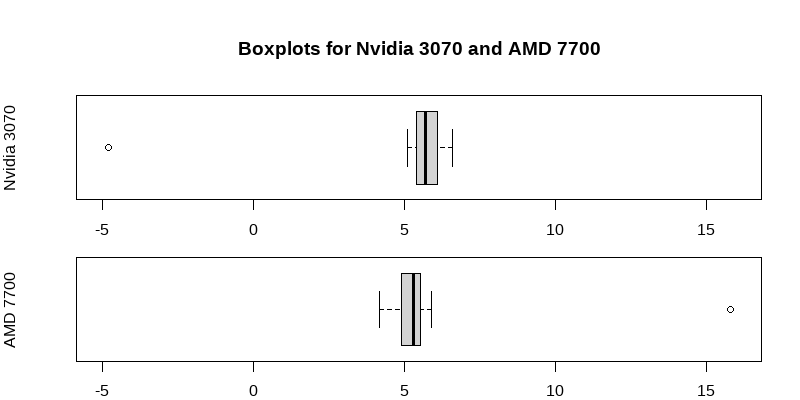
\includegraphics[width=0.75\textwidth]{assets/box_plot}
    \caption{Krabicový graf znázorňující rozložení nárůstu FPS po aplikaci 1.5 patche ve hře "Cyberpunk 2077" pro grafické karty \nvidiaCard\ a \amdCard}
    \label{fig:box_plot}
\end{figure}

\begin{figure}[h!]
    \centering
    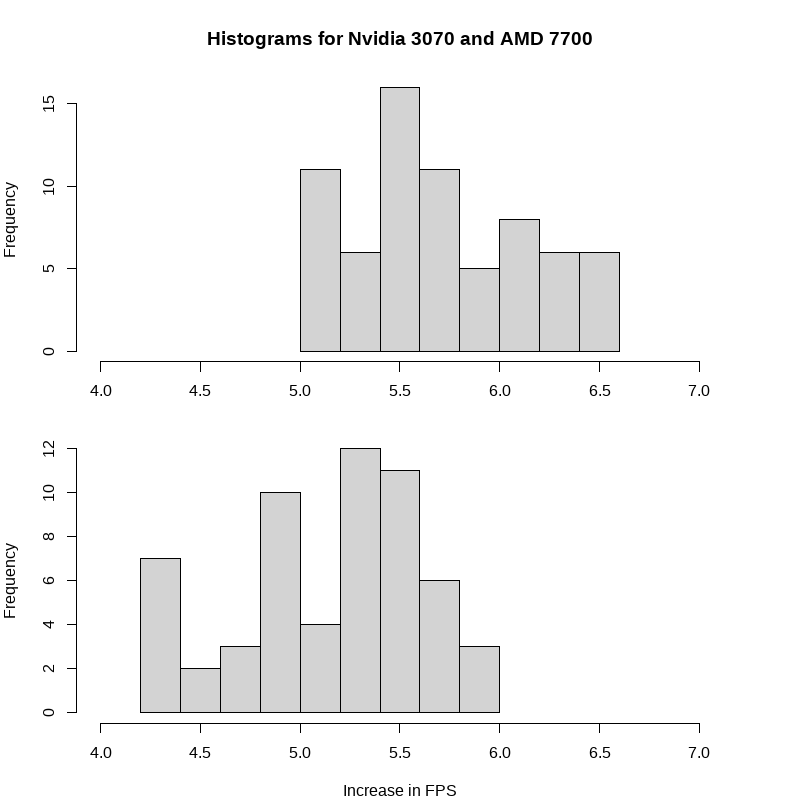
\includegraphics[width=0.75\textwidth]{assets/histogram}
    \caption{Histogram znázorňující rozložení nárůstu FPS po aplikaci 1.5 patche ve hře "Cyberpunk 2077" pro grafické karty \nvidiaCard\ a \amdCard}
    \label{fig:histogram}
\end{figure}

\begin{figure}[h!]
    \centering
    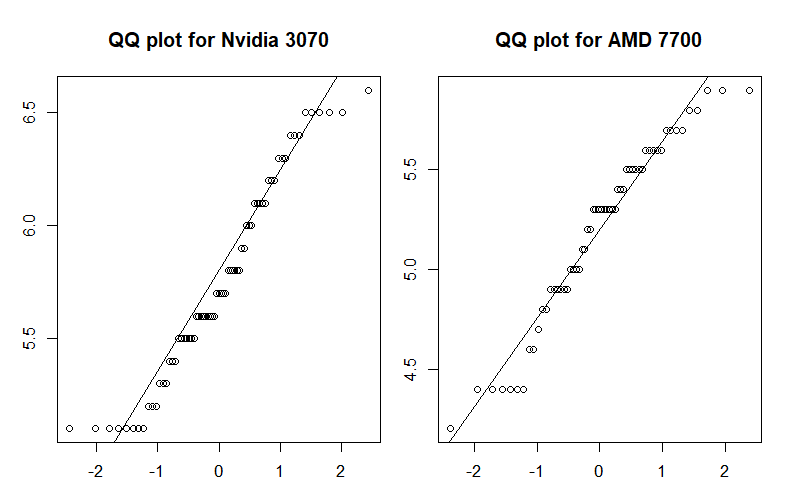
\includegraphics[width=0.85\textwidth]{assets/qq}
    \caption{Q-Q graf znázorňující nárůst FPS po aplikaci 1.5 patche ve hře "Cyberpunk 2077" pro grafické karty \nvidiaCard\ a \amdCard}
    \label{fig:qq}
\end{figure}

\newpage
\subsubsection*{Analýza nárůstu výkonnostních skóre (FPS) po aplikaci 1.5 patche ve hře "Cyberpunk 2077" pro grafickou kartu \nvidiaCard}

Během testu byl zjišťován nárůst FPS pro grafickou kartu \nvidiaCard\ ve hře "Cyberpunk 2077" mezi původním release a verzí s 1.5 patchem
pro \tableValue{\rangeValues}{0} testovacích systémů. Zjištěný nárůst FPS se pohyboval v rozmezí \tableValue{\minValues}{0} FPS
až \tableValue{\maxValues}{0} FPS. Nárůst FPS v testu č. 20 byl na základě metody vnitřních hradeb identifikován jako odlehlé pozorování
a nebude zahrnut do dalšího zpracování. Možné příčiny vzniku odlehlých pozorování jsou: Chyba při testování vzniklá náhlým výkyvem výkonu počítače
nebo chyba hardwaru výpočetní stanice. Dále uvedené výsledky tedy pocházejí z analýzy nárůstů FPS zjištěných u \tableValue{\rangeValues}{2}
testovacích systémů. Průměrný nárůst FPS byl \tableValue{\meanValues}{2} FPS, směrodatná odchylka pak \tableValue{\sdValues}{2} FPS\@.
U poloviny testovacích cyklů nárůst FPS nepřekročil \tableValue{\medianValues}{2} FPS. V polovině případů se nárůst FPS pohyboval v
rozmezí \tableValue{\QfValues}{2} FPS až \tableValue{\QtValues}{2} FPS. Vzhledem k povaze měřené veličiny není variační koeficient vhodnou mírou
pro posouzení variability souboru.

\vspace{1em}
\noindent
Výsledky pro grafickou kartu AMD Radeon RX 7700 XT lze komentovat obdobně.
Nárůst FPS se pohyboval v rozmezí \tableValue{\minValues}{1} až \tableValue{\maxValues}{1} FPS, s průměrným nárůstem \tableValue{\meanValues}{3} FPS a
směrodatnou odchylkou \tableValue{\sdValues}{3} FPS.\@
Za pomocí metody vnitřních hradeb bylo identifikováno odlehlé pozorování v testu č.\ 24, které bylo z analýzy vyloučeno.
Medián nárůstu činil \tableValue{\medianValues}{3} FPS, přičemž polovina výsledků spadala do intervalu \tableValue{\QfValues}{3} až \tableValue{\QtValues}{3} FPS.\@
Opět i zde není variační koeficient vhodným měřítkem variability souboru.

\subsubsection*{Ověření normality nárůstu výkonnostních skóre (FPS) po aplikaci 1.5 patche ve hře "Cyberpunk 2077" pro grafickou kartu \nvidiaCard}

Na základě grafického zobrazení (viz \figref{fig:qq}) u grafické karty \nvidiaCard\ a výběrové šikmosti a špičatosti (viz \tabref{tab:characteristics-summary},
výběrová šikmost a špičatost leží v intervalu (-2, 2)) lze předpokládat, že pozorovaný nárůst FPS má normální rozdělení. Dle pravidla 3$\sigma$ lze tedy očekávat,
že přibližně u 95 \% naměřených nárůstů ve výkonu bude \tableValue{\sigmaValues}{0} FPS až \tableValue{\sigmaValues}{1} FPS\@.

\subsubsection*{Ověření normality nárůstu výkonnostních skóre (FPS) po aplikaci 1.5 patche ve hře "Cyberpunk 2077" pro grafickou kartu \amdCard}

Na základě grafického zobrazení (viz \figref{fig:qq}) u grafické karty \amdCard\ a výběrové šikmosti a špičatosti (viz \tabref{tab:characteristics-summary},
výběrová šikmost a špičatost leží v intervalu (-2, 2)) lze předpokládat, že pozorovaný nárůst FPS má normální rozdělení. Dle pravidla 3$\sigma$ lze tedy očekávat,
že přibližně u 95 \% naměřených nárůstů ve výkonu bude \tableValue{\sigmaValues}{2} FPS až \tableValue{\sigmaValues}{3} FPS\@.

\endinput